\section{Algorithm Design}
\label{sec:alg}

As simultaneously optimizing multiple objectives is difficult, we focus on performance first and discuss how to incorporate online arrivals and fairness considerations later in this section.


%different components in our goals and design functioning parts for fairness, efficiency and performance.


%\subsection{Performance}
%We start considering the Average Completion Time and Makespan objectives via the following model. The model is simplified from the real system, but it tracks the fundamental difference compared to traditional scheduling problem in the system - interchangeability of different computational resource.

%Assume there are $N$ jobs available at the beginning, and they can be executed on either computation resource, GPU ($P_1$) or CPU ($P_2$). For each job $J_j$, the size $\tau_i$ and the executing time on $p_i$ of job $J_j$ can be written as $T_{ijk} = \frac{\tau_i}{s_{ij} k_{ij}}$ where $s_i$ is the speed of job $J_j$ on computation resource $p_i$ and $k_{ij}$ is the parallelization parameter: $ 0\leq k_{ij} \leq 1$ and it requires at any time $t$, $\sum_{j} k_{ij} \leq 1$ for any $i$ . For simplification, we can always assume $s_{2j} = 1$ and scale job size and $s_{1j}$ accordingly. The goal is to minimize ACT.

\subsection{Optimal approach for queued up jobs}

We start with a simplified case where all jobs arrive at the beginning and try to minimize the average job completion time. 
Each job has one configuration for CPU and one for GPU. If a job can only run on GPU or CPU, we can set the processing time on the other resource to be a very large number. 
We assume that each job uses either an entire GPU or an entire CPU, which is further discussed in Section~\ref{sec:system}.

For this simplified problem, we can transform the scheduling and placement problem to a min-cost bipartite matching problem, which can be solved efficiently~\cite{galil1988n}.
Specifically, our algorithm consists of three steps: (i) generate input for the min-cost bipartite matching problem based on job information; (ii) solve the matching problem to obtain a solution; (iii) convert the solution to a feasible scheduling and placement. 


%\xiao{todo: add figure and explanation first for readers to understand better ---- explanation to be added}

\paragraph{Generate input for the matching problem.}
%Our key observation is that for each resource (a CPU or a GPU), a job scheduled as the $k$-th last one contributes $k$ times its processing time to the total job completion time. This is illustrated in Figure~\ref{fig:alg_idea}. In this case, we have three jobs of sizes 3, 4, and 5 to be scheduled on one resource. If we schedule in the order given in Figure~\ref{fig:alg_idea1}, the completion time is 3, 7, and 12, resulting in a total completion time of 22. 
%Another way to calculate the total completion time is using Figure~\ref{fig:alg_idea2}. While Job 1 is being processed, the waiting time of Job 2 and 3 is aggregated vertically. As the Job 1 is scheduled to be the third last one, i.e., there are two jobs waiting, it contributes 3 times (two from waiting time of Jobs 2 and 3, and one from Job 1's own processing time) to the total completion time, which is 9. Similarly, as Job 2 is scheduled as the second last job, it contributes twice its processing time, which is 8. Finally, Job 3 is the last job, so it contributes only its processing time 5. The sum is also 22.


Our observation is that for each resource (a CPU or a GPU), a job scheduled as the $k$-th last one contributes $k$ times its processing time to the total job completion time.
Assume we have three jobs of sizes 3, 4, and 5 to be scheduled on one resource.
If we schedule in the order, their completion times are 3, 7, and 12, resulting in a total completion time of 22. 
There is another way to calculate the total completion time based on the waiting times.
%While Job 1 is being processed, the waiting time of Job 2 and 3 is aggregated.
As the Job 1 is scheduled to be the third last one, i.e., there are two jobs waiting, it contributes 3 times (two from waiting times of Jobs 2 and 3, and one from Job 1's own processing time) to the total completion time, which is 9.
Similarly, Job 2 contributes twice its processing time, which is 8.
Job 3 is the last job and contributes only its processing time 5.
The sum is also 22.  

%\begin{figure}[h]
%	\centering
%	\subfloat[3 jobs are scheduled on this machine.] {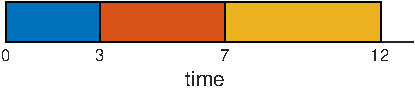
\includegraphics[width=0.45\linewidth]{figs/alg_ex1} \label{fig:alg_idea1}}    \hspace{0.0in}
%	\subfloat[The total processing time on this machine can be viewed as the total area counted vertically.] {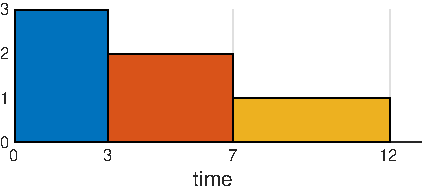
\includegraphics[width=0.45\linewidth]{figs/alg_ex2} \label{fig:alg_idea2}} 
%	\caption{Our key observation: a job scheduled as the $k$-th last one contributes $k$ times its processing time to the total job completion time.}
%	\label{fig:alg_idea}
%\end{figure}

% The idea is the following: let $S$ be a schedule and suppose job $J_j$ is executing on resource $P_i$ with full parallelization, assume there are $k-1$ jobs scheduled after $J_j$ on $P_i$. Let $t(S)= \sum_j^n f(J_j)$ be the total completion time based on schedule $S$, where $f(J_j)$ is the completion time for job $j$. (Add citation)


This observation allows us to obtain the contribution of a job placed on machine $i$ as the $k$-th last job to the total completion time. %Here $k$ is counted backwardly, meaning $k_{th}$ last job on machine $i$. 
Consider a simple example with 2 machines (1 CPU and 1 GPU) shared by 3 jobs. The job processing time can be represented by the following processing time matrix $P$ where each row contains processing time on CPU and GPU. In this matrix, the first row represents that Job 1 takes 3 minutes on GPU or 4 minutes on CPU. The size of $P$ is $n\times m$ for $n$ jobs over $m$ machines.

$$
P = \begin{bmatrix}
3 & 4 \\
4 & 6 \\
5 & 10\\
\end{bmatrix}
$$

Based on the processing time matrix $P$, we can generate the following cost matrix $$Q = \begin{bmatrix}
P & 2\times P &\cdots& n\times P
\end{bmatrix}. $$
The size of $Q$ is $n\times (nm)$.

For our example, 
% $$
% Q = \begin{bmatrix}
% 3 & 4 & 6 & 8 & 9 & 12\\
% 4 & 6 & 8 & 12 & 12 & 18\\
% 5 & 10 & 10 & 20 & 15 & 30\\
% \end{bmatrix}
% $$
$$Q = \bordermatrix{
~ &(G,1) & (C,1) & (G,2) & (C,2) & (G,3) & (C,3) \cr
~& 3 & 4 & 6 & 8 & 9 & 12 \cr
~& 4 & 6 & 8 & 12 & 12 & 18 \cr
~& 5 & 10 & 10 & 20 & 15 & 30 \cr
}$$

The element $(j,(i,k))$, corresponding to $(j,m*(k-1)+i)$ in the matrix,  represents the cost of scheduling job $j$ at machine $i$ (1 stands for GPU, and 2 stands for CPU) as $k$-th last job. For example, the entry $(2, (1,3))$ represents Job 2 contributes 12 minutes processing time if it is placed as the third last job on GPU. %We can observe that $Q$ can be written as where $P$ is the processing time matrix given above. 

\begin{figure}[h]
\centering
\begin{tikzpicture}[
      mycircle/.style={
         circle,
         draw=black,
         fill=gray,
         fill opacity = 0.3,
         text opacity=1,
         inner sep=0pt,
         minimum size=20pt,
         font=\small},
      myarrow/.style={-Stealth},
      node distance= 0.3cm and 1.0cm
      ]
      \node[mycircle] (c1) {$G1$};
      \node[mycircle,below=of c1] (c2) {$C1$};
      \node[mycircle,below=of c2] (c3) {$G2$};
      \node[mycircle,below=of c3] (c4) {$C2$};
      \node[mycircle,below=of c4] (c5) {$G3$};
      \node[mycircle,below=of c5] (c6) {$C3$};
      \node[mycircle,above right= 1cm and 5cm of c3] (c7) {$Job1$};
	\node[mycircle,below= 1.5cm of c7] (c8) {$Job2$};
    \node[mycircle,below= 1.5cm of c8] (c9) {$Job3$};
     \draw [myarrow] (c1) -- (c7);
     \draw [blue,myarrow,thick] (c2) --node [font=\fontsize{12}{12}\sffamily\Large\bfseries\selectfont,above] {4} (c7);
     \draw [myarrow] (c3) -- (c7);
     \draw [myarrow] (c4) -- (c7);
     \draw [myarrow] (c5) -- (c7);
     \draw [myarrow] (c6) -- (c7);
     \draw [myarrow] (c1) -- (c8);
     \draw [myarrow] (c2) -- (c8);
     \draw [blue,myarrow,thick] (c3) --node [font=\fontsize{12}{12}\sffamily\Large\bfseries\selectfont,above left = -0.4cm and 0.7cm] {8} (c8);
     \draw [myarrow] (c4) -- (c8);
     \draw [myarrow] (c5) -- (c8);
     \draw [myarrow] (c6) -- (c8);
     \draw [blue,myarrow,thick] (c1) --node [font=\fontsize{12}{12}\sffamily\Large\bfseries\selectfont,below right=0.9cm and 1.3cm] {5} (c9);
     \draw [myarrow] (c2) -- (c9);
     \draw [myarrow] (c3) -- (c9);
     \draw [myarrow] (c4) -- (c9);
     \draw [myarrow] (c5) -- (c9);
     \draw [myarrow] (c6) -- (c9);
    \end{tikzpicture}
    \caption{The corresponding min-cost bipartite matching problem.}
        \label{fig:bipartite}
\end{figure}

% We can rewrite $t(S)$ in such a way as to isolate all terms which depends on $\theta_{ij} = \frac{\tau_j}{ s_i}$, so that $t(S) = k\theta_{ij} $ plus $(n-1)$ other terms that does not containing $\theta_{ij}$. If $J_j$ runs at last $r$ of all jobs on $P_i$, then the coefficient of $\theta_{ij}$ is $r$, so we have a matrix of matrix $$ Q = \begin{bmatrix}
% [\theta_{ij}] \\
% [2\theta_{ij}] \\
% \cdots \\
% [n\theta_{ij}] \\
% \end{bmatrix} $$, where $[\theta_{ij}]$ is a $2\times n$ matrix representing the fully parallized processing time on different resources. so $Q$ is a $2n \times n$ matrix.

% A set of $n$ elements $\{q_{i_1 1},q_{i_2 2},\cdots,q_{i_n n} \}$ in $Q$ is called a feasible set if no 2 elements are in the same row. The optimal solution of $t(S)$ is equivalent to the minimum cost of feasible set of $Q$. 


\paragraph{Solve the matching problem.}
Given the matrix $Q$, we can formulate the problem into a min-cost bipartite matching problem in Figure~\ref{fig:bipartite} as following: %\todo{figure reference does not work} \xiao{fixed}

On the right side of the bipartite graph, each node represents a job. For our example, there are three jobs. Because each job needs to be scheduled on one machine, it has a demand of 1 unit. On the left side, each node represents a position on a machine. As we have two machines (one CPU and one GPU) and 3 jobs, we need at most three positions for each machine. For instance, G2 represents the second last position on GPU. Because each position on a machine can serve one job at most, it has a supply of 1 unit. 

Each edge has a capacity of 1 and there is a one-to-one correspondence between the cost of using that edge and the entry from the matrix $Q$ we generated. For example, the cost from $G2$ to node $Job2$ is the entry at the second row and $(G,2)$ column, which is 8.

This min-cost bipartite matching problem can be solved in polynomial time with standard network flow algorithms or Hungarian method~\cite{orlin1993faster, kuhn1955hungarian}. In the example, the optimal cost is 17 and the matching is shown in a matrix $M$. Three highlighted edges in Figure~\ref{fig:bipartite} are active to feed the demand. 
%\xiao{new: and the corresponding matching matrix $M$ is the following}
$$M = \bordermatrix{
~ &(G,1) & (C,1) & (G,2) & (C,2) & (G,3) & (C,3) \cr
~& 0 & 1 & 0 & 0 & 0 & 0 \cr
~& 0 & 0 & 1 & 0 & 0 & 0 \cr
~& 1 & 0 & 0 & 0 & 0 & 0 \cr
}$$
\paragraph{Convert the matching solution to job scheduling.}

The solution from the matching problem is converted as follows. %We consider all active edges, from the 1-1 correspondence between the edges and matrix $Q$, we can find the entry which equals to the cost of the edge. 
Each edge picked by the matching algorithm correspond to the scheduling and placement of a job. For instance, the edge between $Job2$ and $G2$ is picked, meaning Job 2 is scheduled on GPU as the second last job. Similarly, $Job3$ is connected to $G1$, meaning it is scheduled on GPU as the last job. $Job1$ is connected to $C1$, so it is scheduled on CPU as the last job. 
Combined the information, our algorithm places Job2 and Job 3 on GPU and Job 2 is scheduled before Job 3, while Job 1 is placed on CPU as the only job. 
%The entry from the matrix provides all information we need for scheduling: the row number provides the job ID to be scheduled, the column number provide the machine ID and the position of that job in the scheduling.
%In the example, the corresponding entries are $[3,(G,1)]$, $[1,(C,1)]$,$[2,(G,2)]$. So Job 3 will be scheduled as the last job on GPU, job 1 will be scheduled on CPU as the last job, while job 2 will be scheduled on GPU as the second last job. 
This scheduling and placement are shown in Figure~\ref{fig:FS_ex}.

\begin{figure}[h]
	\centering
	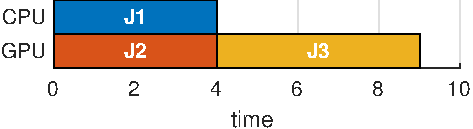
\includegraphics[width=0.7\linewidth]{figs/FS_ex}
	\caption{The scheduling from the corresponding min-cost bipartite matching problem, with total completion time of 17.}
	\label{fig:FS_ex}
\end{figure}

%We begin with the case with only 1 computation resource: CPU. 


%\begin{restatable}[]{lem}{SJF} If we sort all jobs based on $\tau_j$, then SJF is optimal and we always set $k_j = 1$. \end{restatable}

%This can be proved via 2 steps: first is to show that sharing the resource at any time is unnecessary via resizing the jobs; second is to show that SJF is optimal via exchange argument.

%When there are 2 resources, we can also find the optimal scheduling.



Regarding the performance of this transformation, each scheduling and placement solution corresponds to a feasible solution of the matching problem. To see this, each job has been placed on one and only one machine, meaning the demand of each job node in the matching problem has been met. In addition, no jobs have the same order at the same machine, so the supply of each (machine, order) node in the matching problem is at most 1. 
%To see the correspondence, consider any valid schedule for the original problem, then for each job $j$, it has an assigned resource $r$ and a relative order $k$ on that machine, then the two number corresponds to a number in the matrix $Q(2k-2+r,j)$, and obviously, no jobs have the same order at the same machine and each job can be scheduled only once, so any feasible schedule corresponds to a feasible set in $Q$. 

Conversely, any feasible solution to the matching problem corresponds to an extended scheduling problem with possibly dummy jobs. 
To do this, we first place jobs based on the edges picked by the matching problem. Then we fill each gap in the positions by a dummy job. For instance, if only $G1$ and $G3$ are picked, we insert a dummy job for $G2$. 

Clearly, the insertion of dummy jobs always increases the total completion time. Therefore, there is no dummy job in the optimal solution of the matching problem. In other words, for any solution with dummy jobs, we can remove the dummy jobs and move all following jobs forward to finish them earlier, which gives another feasible solution with better completion time. 
Therefore, we have the following optimality result.

\begin{restatable}[]{lem}{SJF} When all jobs arrive at the same time, the optimal solution can be found in polynomial time by solving a corresponding min-cost bipartite matching problem. \end{restatable}

%based on their assigned order on the matrix $Q$, and fill in dummy jobs with 0 processing time if no job is using that assigned slot, by doing this, we can generate a schedule composite of both jobs from set $J$ and dummy jobs.  Next, we can show that, for any feasible set that corresponds to a schedule with dummy jobs, it is not an optimal feasible set. Consider any job $j^*$ that follows a dummy job in the schedule, and assume its corresponding row in the matrix is $x$, then clearly, any number in row $x-M$ is not picked, as otherwise there won't be a dummy job before $j^*$. Then clearly we can pick job $j^*$ at row $x-M$ instead of row $x$, and from the definition of $Q$, the cost from row $x-M$ for job $j^*$ is smaller than the cost from row $x$, so it is not a optimal solution. In other words, any optimal feasible set corresponds to a feasible schedule with non-dummy jobs.

%Combine two parts together, we have the following optimality.

% \begin{algorithm}[H]
% \small
% \caption{Primitive \name without arrivals}
% \label{alg:greedy}
% \begin{algorithmic}[1]
% 	\While{ a machine $i$ becomes available}
%     \ForAll{job $j$ in the waiting queue}
%     \State Add processing time of job $j$ to the matrix $P$
%     \EndFor
%     \State Generate the delay matrix $D$;
%     \State Generate the matrix $Q$ using  equation \eqref{eq:generate_cost}
%     \State Solve the min cost matching problem based on $Q$ to generate the matching matrix $M$
%     \For{k = $J$:1}
%     \State Find the first Job $j$ such that $M(j,(i,k))=1$ and place Job $j$ on machine $i$. 
% %     \For {w = $1:J$}
% %     \If{entry $(w,(i,k))$ is picked}
% %     \State add job $w$ to machine $i$
% %     %\State Update $\omega_i$ \todo{do we need this line?}
% %     %\State Break
% %     \EndIf
% %     \EndFor
%      \EndFor
%     \State break;
%     \EndWhile
% %     \State Generate matrix $Q$;
% %     \State Solve a min-cost bipartite matching problem for matrix $Q$;
% %     \State Retrieve scheduling from the solution

% %\todo{make it more general so we can schedule multiple jobs each time.}
% \end{algorithmic}
% \end{algorithm}

%\xiao{I moved this algorithm to 3.1 and edit it to schedule all jobs at the beginning (as there is no arrivals)}
\begin{algorithm}[H]
\small
\caption{Primitive \name without online arrivals}
\label{alg:greedy}
\begin{algorithmic}[1]
    \State Generate the cost matrix $Q$
%    \State Generate the cost matrix $Q$;
    \State Solve the min-cost matching problem defined by $Q$ to get the matching matrix $M$
    \For{$j = 1 : n$}   \Comment{$n$ is the total \# of jobs}
    \For{$i = 1: m$} \Comment{$m$ is the total \# of machines}
    \For{$k = n : 1$}
    \If{$M(j,m(k-1)+i) = 1$} \Comment{Job $j$ is scheduled on machine $i$ as the $k$-th last job}
    \State Add job $j$ to the queue from machine $i$
    \EndIf
%     \For {w = $1:J$}
%     \If{entry $(w,(i,k))$ is picked}
%     \State add job $w$ to machine $i$
%     %\State Update $\omega_i$ \todo{do we need this line?}
%     %\State Break
%     \EndIf
%     \EndFor
	\EndFor
     \EndFor
     \EndFor
%     \State Generate matrix $Q$;
%     \State Solve a min-cost bipartite matching problem for matrix $Q$;
%     \State Retrieve scheduling from the solution

%\todo{make it more general so we can schedule multiple jobs each time.}
\end{algorithmic}
\end{algorithm}





\subsection{Handling online arrivals}
The algorithm described the from previous section requires all jobs to arrive at the beginning. When there are arrivals over time, even if the arrival times are known beforehand, the problem is APX-hard under multiple configurations~\cite{hoogeveen1998non}.


% ~\todo{any citation or reduction? What happens if there is only one configuration for each job?}. Even if there is only one configuration for each job, the problem is NP-hard with preemption allowed~\cite{Bellenguez.ea:15:A-Note-on-NP-Hardness}.

In \name, we extend our idea in the previous section to incorporate arrivals by updating the scheduling and placement over time. This can be done frequently, e.g., whenever there is a resource becomes available, or once a while either periodically or aperiodically.  

We focus on the case where preemption is not allowed and the scheduler has no information about future arrivals. The major difference with arrivals over time is that when we generate a new scheduling, some machines are occupied so new jobs need to wait until the current jobs to finish. We use both the arrival time of new jobs and the available time of machines to adjust the cost matrix $Q$ for the matching problem. 

%To proper adjust the cost matrix, we need to record both the arrival time of the waiting jobs and the available time of all machines.



Consider the example in Figure~\ref{fig:arrival_ex}. Assume we generated a schedule at time $0$ and a job was placed on the machine $i$, which is expected to finish at time $10$. In other words, the available time of machine $i$ is $\omega_i = 10$. 
Job $j$ arrives at time $4$ but the scheduler was not triggered at that time. 
At time $T=6$, we want to update the schedule, while machine $i$ is still busy. 
For Job $j$, if it is scheduled as the next job on machine $i$,its (expected) completion time comes from two parts: a waiting time of $(\omega_i - a_j)=6$ and the processing time $p_{ji}=5$. This gives an expected completion time of 11. 



%Assume when Job $j$ arrives, the scheduler was not triggered and the scheduler is triggered at time $T=6$. %at current time $T=6$, the schedule will be regenerated.
%However, due to the non-preemptive property, machine $i$ is still running, and it is expected to finish the current job at time $\omega_i = 10$.
%If the schedule returns back a solution and indicates that Job $j$ is scheduled next on machine $i$, the total completion time of Job $j$ come from 2 parts: waiting time $(\omega_i - a_j)=6$ and processing time $p_{ji}=5$, with a total flow time 11.



\begin{figure}[h]
	\centering
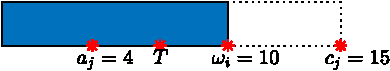
\includegraphics[width=0.7\linewidth]{figs/arrival_ex}
	\caption{An illustration example that shows the impacts of online arrivals and available time of a machine.}
	\label{fig:arrival_ex}
\end{figure}



Motivated by this, we define delay matrix  $D(j,i) = \omega(i) - a(j)$, where $a(j)$ is the arrival time of job $j$, and $\omega(i)$ is the earliest available time of machine $i$ when it finishes its currently allocated job(s). If machine $i$ is idle, then $\omega(i) = T$, where $T$ is the current time. The cost matrix $Q$ is calculated by the following: 

\begin{equation}
Q = \begin{bmatrix}
P & 2P &\cdots& nP
\end{bmatrix} + \begin{bmatrix}
D & D &\cdots& D
\end{bmatrix}
\label{eq:generate_cost}
\end{equation}



%\todo{the following part is hard to understand in the current form} \xiao{I added another example above}
% So it is important to know when the node will finish its current running job. To do so, we define delay matrix  $D(i,j) = \omega(i) - a(j)$, where $a(j)$ is the arrival time of job $j$, and $\omega(i)$ is the earliest available time of machine $i$ when it finishes its current job.  as $a(j) \leq $ current time and $\omega(i) \geq $ current time, so $D(i,j)$ is non-negative. Consider in Figure \ref{fig:flowex1}, if 2 new jobs arrive at time 2 and 3 separately. Then $$D = \begin{bmatrix}
% 4 & 3 \\
% 1 & 0 \\
% 3 & 2 \\
% \end{bmatrix}
% $$

% \begin{figure}[h]
% 	\centering
% 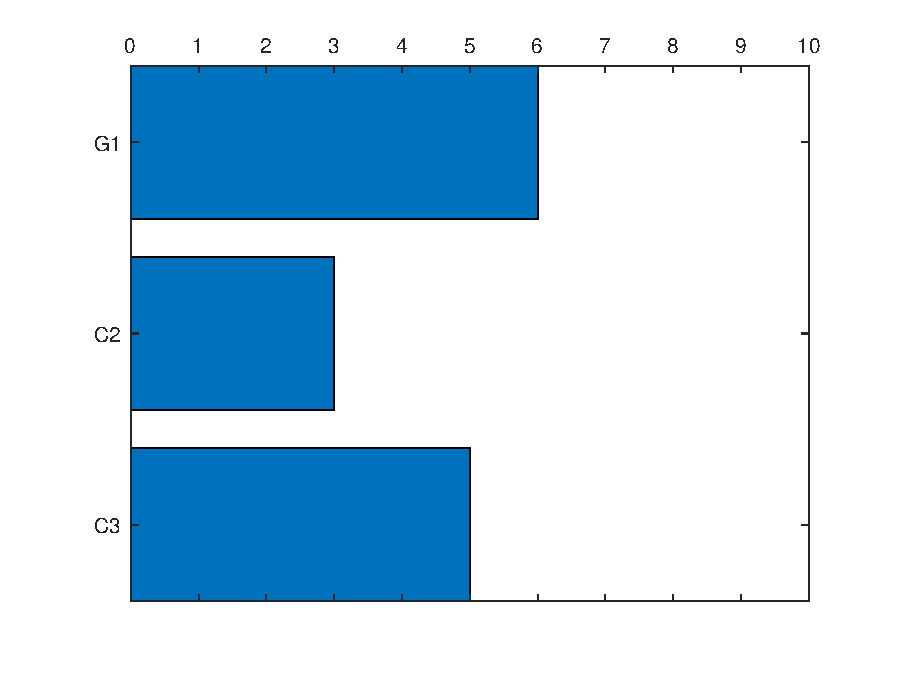
\includegraphics[width=0.8\linewidth]{figs/alg_1new}
% 	\caption{At time 3, $\omega = (6,3,5)$, if no job is being scheduled since time 3, then at time 5, $\omega = (6,5,5)$}
% 	\label{fig:flowex1}
% \end{figure}


% Assume the $P$ is the following:
% $$P = \begin{bmatrix}
% 1 & 1 \\
% 10 & 10 \\
% 10 & 10 \\
% \end{bmatrix}
% $$
% Machine 1 is GPU and machine 2 and 3 are CPU. Consider a larger matrix $Q$:
% \begin{equation}
% Q = \begin{bmatrix}
% [D] \\
% [D] \\
% \cdots \\
% [D] \\
% \end{bmatrix}
%  + \begin{bmatrix}
% [P] \\
% [2P] \\
% \cdots \\
% [NP] \\
% \end{bmatrix}
% \label{eq:cost_mat}
% \end{equation}
% where $N$ is the total number of jobs from users whose fairness score is within $\alpha$ fraction.


% Using an example with 2 jobs from matrix $D$ and $P$, consider at time 3, we have $$ Q = \begin{bmatrix}
% 5 & \textcircled{4}\\
% 11 & 10 \\
% 13 & 12 \\
% \textcircled{6} & 5 \\
% 21 & 20\\
% 23 & 22
% \end{bmatrix}  $$

% The schedule method will pick 2 circled numbers 4 and 6 (or 5,5 it is the same). The entry of number 4 is (1,2), it represents that job 2 is last one scheduled on machine 1. The entry of number 6 is (4,1), it represents that job 1 is second last one scheduled on machine 1.  

% Since no job will be scheduled on current empty machine 2, the scheduler will do nothing and wait until another job arrives or a new machine becomes free.

%\todo{Add the Allox algorithm formal description without fairness consideration} \xiao{added}

%\todo{xiao: add a part on scheduling with more than 1 machine}

%\subsection{Incorporation jobs with different resource requirement}


%NP-hardness from \cite{drozdowski1996scheduling}, NP-hard even there are only 2 identical machines and job demand is either 1 or 2.

%idea: 





% \subsubsection{Makespan}

% For single computation resource, the problem is trivial - any non-idle scheduler will be optimal for makespan objective, no ordering or parallelism need to be considered.

% With 2 computation resource, the problem is NP-hard from 2-partition. However, there are algorithms that is 2-approximation. The idea is to consider a feasibility problem on a bipartite graph (consider each machine has the same budget) and solve the integer programming it using iterative rounding.

% However, with 2 resources, we can have simple greedy algorithm that also achieve good approximation: (high-level idea: we are doing optimally in placement, and try to push to optimality in balancing the load)

% \begin{algorithm}[H]
% \small
% \caption{Makespan Optimizer}
% \label{alg:greedymakespan}
% \begin{algorithmic}[1]
%     \State Schedule all jobs in CPU in any order with fully parallelization
%     \State Let $w_j = \theta_{1j}-\theta_{2j}$, define $W$ as the set of all $w_j$, sort $W$ decreasingly
%     \State Move jobs from CPU to GPU based on set $W$ to find a minimized makespan
% \end{algorithmic}
% \end{algorithm}


% \begin{restatable}[]{lem}{SJF} Algorithm \ref{alg:greedymakespan} is $2-$approximation for makespan.\end{restatable}

% Let $L_1(j)$ be the length of all jobs scheduled on CPU when first $j$ jobs are moved to GPU, $L_2(j)$ be the length of all jobs scheduled on GPU when first $j$ jobs are moved to GPU. Firstly we show that $ \min_i(L_i(j)) \leq OPT$ for any $j$, where $OPT$ is the optimal solution of makespan.

% Let the optimal schedule be $S$. In $S$, let the set of jobs that are scheduled on CPU be $S_1$, let the set of jobs that are scheduled on CPU be $S_2$. Then by contradiction, we have 

% $$ \max (\sum_{k \in S_1} \theta_{1k}, \sum_{k \in S_2} \theta_{2k} ) < \min (\sum_{k = j+1}^n \theta_{1k}, \sum_{k=1}^j\theta_{2k}) $$, which can be decomposed into 4 inequalities. Then we can prove that at least 1 inequality cannot hold.

% Then we consider $r$ and $r+1$ in $K$ where the type of resource of the longer length changes. 

% Then clearly one of the case is our solution, and we have $L_{alg} \leq OPT + \min{ \theta_{i(r+1)}}$ , and $\min_i { \theta_{i(r+1)}} \leq OPT$. So this leads to a 2-approximation.

% \todo{ If we set the placement based on Alg 2 and reorder within each resource based on processing time, will this algorithm has an approximation ratio for ACT?}



% \subsection{Makespan}

% Makespan cares more about the actual gain switching from GPU to CPU. (for example, consider a job with processing time (1,10) and another (10,100), they have same $\beta$, but the gain contributing to makespan is largely different. 

% At a high level, without considering the resource capacity, we should schedule jobs to GPU where $\delta$ is larger.

% If we have to consider the capacity, then we also needs to pack the jobs based on some similarity approach.





% \subsection{Average Completion Time}

% ideally, to minimize average completion time, we should always schedule shorter jobs first. As every job has 2 configurations, the simplest approach is that we sort all processing time and pick jobs based on processing time increasingly.





